%%%%%%%%%%%%%%%%%%%%%%%%%%%%%%%%%%%%%%%%%%%%%%%%%%%%%%%%%%%%%%%%%%%
%%% Documento LaTeX 																						%%%
%%%%%%%%%%%%%%%%%%%%%%%%%%%%%%%%%%%%%%%%%%%%%%%%%%%%%%%%%%%%%%%%%%%
% Título:		Capítulo 2
% Autor:  	Ignacio Moreno Doblas
% Fecha:  	2014-02-01, actualizado 2019-11-11
% Versión:	0.5.0
%%%%%%%%%%%%%%%%%%%%%%%%%%%%%%%%%%%%%%%%%%%%%%%%%%%%%%%%%%%%%%%%%%%
% !TEX root = A0.MiTFG.tex
\chapterbegin{Especificaciones}
%\label{chp:Utiliz}
\minitoc
\clearpage

\section{Diagramas}

En este apartado se engloban todos los diagramas realizados a la hora de definir el proyecto y su alcance.

    \subsection{Contexto}
     
    En la figura \ref{fig:CtxDiagram} se puede observar el entorno circundante al proyecto, representado por un diagrama de contexto. El bloque correspondiente al proyecto en sí es el denominado como “Entorno pruebas de algoritmos ECG”, los otros bloques representan elementos relacionados con los que se interacciona de una forma u otra. 

    Este diagrama resulta de bastante ayuda a la hora de establecer los casos de uso que serán detallados más adelante, pues al visualizar de un solo vistazo todo el entorno circundante al producto se pueden descubrir nuevas interacciones que habrían sido ignoradas de otra forma.        

    \begin{figure}[H]  
        \centering
            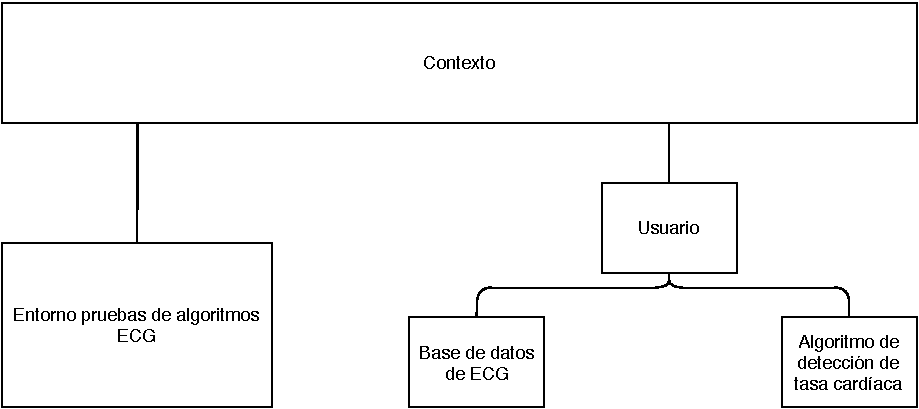
\includegraphics[width =\linewidth]{figuras/ContextDiagram.pdf}
        \caption{Diagrama de contexto}
        \label{fig:CtxDiagram}
    \end{figure}

    \subsection{Casos de uso}

    Una vez establecido el contexto en el que se desenvuelve el proyecto se pueden establecer los casos de uso. De nuevo se realiza un esquema para poder visualizarlos como conjunto. Este esquema puede verse en la figura (TODO: Cita figura), en él se muestran las acciones que podría llevar a cabo el usuario una vez el proyecto esté finalizado, aunque será tarea futura determinar cuales gozan de mayor prioridad, pues no todas son iguales de fundamentales a la hora de llevar a cabo el objetivo principal del proyecto.

    \begin{figure}[H]  
        \centering
            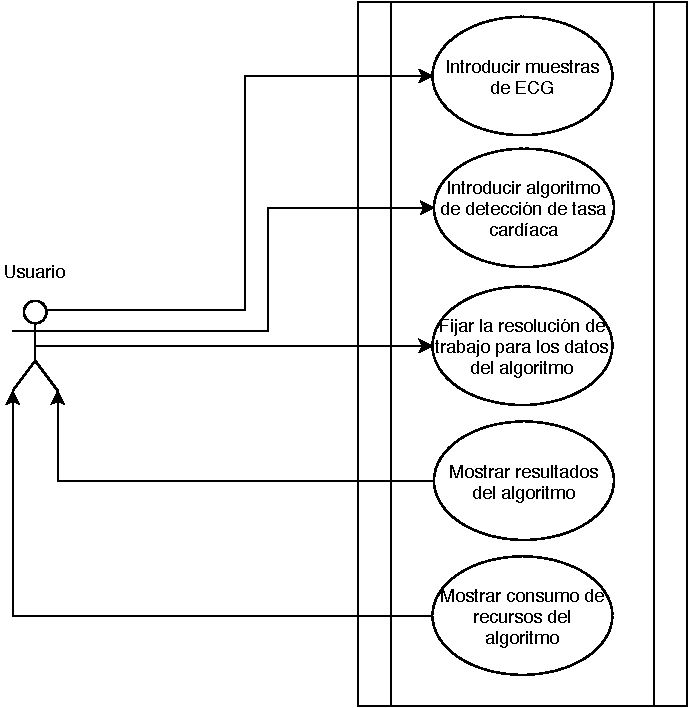
\includegraphics[width =0.7\linewidth]{figuras/UseCasesDiagram.pdf}
        \caption{Diagrama de casos de uso}
        \label{fig:UseCasesDiagram}
    \end{figure}

    Estando aclaradas estas interacciones ya resulta posible comenzar a establecer los requisitos del proyecto, sin embargo primero se debería establecer conceptualmente el flujo de trabajo que se llevará a cabo para el testeo de los algoritmos.

    \subsection{Flujo}

    De forma muy simplificada se puede observar en la figura (TODO: Citar figura) el flujo de trabajo del entorno de pruebas. Este diagrama es útil para tener en mente en todo momento el objetivo del proyecto en su versión más simplificada.

    \begin{figure}[H]  
        \centering
            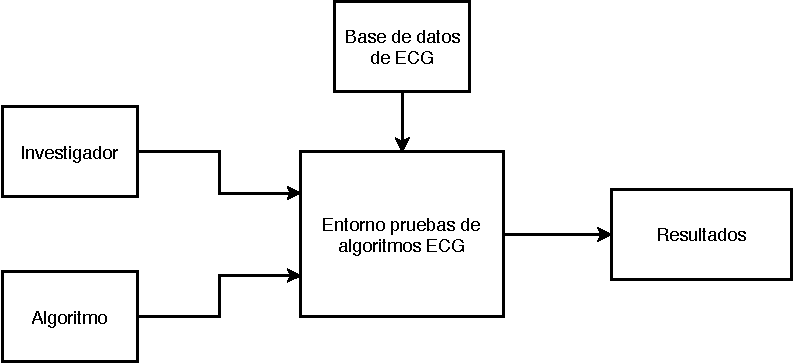
\includegraphics[width =\linewidth]{figuras/BlocksDiagram.pdf}
        \caption{Diagrama de bloques}
        \label{fig:BlocksDiagram}
    \end{figure}
    \clearpage


\section{Requisitos generales}

    Con la ayuda de los diagramas realizados se establecen los siguientes requisitos para cumplir con el objetivo establecido:
     
    \begin{scriptsize}
    \begin{longtable}{|p{0.05\linewidth}|p{0.21\linewidth}|p{0.3\linewidth}|p{0.3\linewidth}|p{0.03\linewidth}|}
        \hline
        ID & Requisito & Descripción & Prueba & Prio \\ \hline
        \endfirsthead
        %
        \endhead
        %
        \hline
        \endfoot
        %
        \endlastfoot
        %
        1 & Panel de control & El proyecto debe disponer de un panel de usuario intuitivo para llevar a cabo las pruebas &  & 1 \\ \hline
        1.1 & Introducir señal de prueba & Al panel de control se le debe proveer una señal de ECG formateada específicamente para poder probar el algoritmo deseado & Introducir un ECG extraido de alguna base de datos y comprobar que los valores de las muestras enviados se corresponden & 1 \\ \hline
        1.2     & Observar el comportamiento del algoritmo & Al panel de control se le debe proveer de gráficas de salida que muestren el estado de la señal procesada. & Observar las gráficas de salida y comprobar con un algoritmo predecible que el resultado obtenido es el deseado & 2 \\ \hline 
        1.3     & Resultados & El panel de control debe ser capaz de mostrar al usuario los siguientes elementos: &  &  \\ \hline
        1.3.1   & Frecuencia cardiaca instantanea & El panel deberá mostrar la frecuencia cardíaca instantanea medida por el algoritmo a testear. & Comprobar que el dato enviado por la aplicación de pruebas y el recibido por el panel son el mismo. La precisión de este no es un requisito pues dependerá del algoritmo con el que se esté trabajando. & 1 \\ \hline
        1.3.2   & Picos detectados & El panel deberá mostrar nformación sobre los picos R detectados y sus posiciones, para facilitar la evaluación del algortimo & Al igual que la prueba anterior, se debe garantizar la coherencia de los datos entre la aplicación y el panel de usuario. La validez de estos dependerá del algoritmo. & 1 \\ \hline
        1.3.3   & Utilización del procesador instantanea & El panel deberá mostrar de forma instantanea el uso de CPU que corresponde al proceso del algortimo de la forma más aproximada posible &  & 2 \\ \hline
        1.3.4   & Utilización de memoria instantanea & El panel deberá mostrar el uso de memoria en cada momento de la forma más aproximada posible &  & 2 \\ \hline
        1.3.5   & Fiablidad del algoritmo & El panel deberá mostrar la fiablilidad (bien visual o bien en forma de tasas de falsos positivos y negativos) del algoritmo. & Contrastar con las anotaciones de la base de datos. & 2 \\ \hline
        1.4     & Resolución muestras & El panel deberá poder configurar la resolución empleada para las muestras en la aplicación, ofreciendo al usuario cierto control sobre la cantidad de muestras simultaneas con las que su algoritmo podrá trabajar. &  & 2 \\ \hline
        2       & Aplicación de pruebas & El proyecto debe disponer de una aplicación encargada de simular el comportamiento de un supervisor de eventos cardíacos introduciendo el algortimo de detección de tasa cardíaca deseado. &  & 1 \\ \hline
        2.1     & Protocolo de comunicación & La aplicación debe ser capaz de recibir los datos desde el panel de usuarios y devolver los resultados procesados. & El correcto funcionamiento del resto de requisitos es preba suficiente para este. & 1 \\ \hline
        2.2     & Entrada de datos en tiempo real & La aplicación debe enviar y recibir los datos en tiempo real para emular las condiciones de funcionamiento de un SEC. & Comprobar que la aplicación es capaz de recibir datos paulatinamente y devolverlos. & 1 \\ \hline
        2.2.1   & Simular la entrada de datos por el ADC & La aplicación debe simular la adquisición de datos mediante un conversor analógico digital. Emulando el funcionamiento de un supervisor real. & Comprobar que el acceso a esos datos está controlado con un Timer, como si del ADC se tratase. & 2 \\ \hline
        2.3     & Interfaz para el algoritmo & La aplicación debe disponer de una interfaz, dentro de la cual se pueda encapsular el algoritmo de detección de tasa cardíaca que el usuario desee probar. & Implementar dos algoritmos diferentes sin necesidad de modificar nada fuera de la interfaz. & 1 \\ \hline
        2.4     & Resolución muestras & La aplicación debe ser capaz de modificar la resolución empleada para las muestras en la aplicación, ofreciendo al usuario cierto control sobre la cantidad de muestras simultaneas con las que su algoritmo podrá trabajar. & Comprobar que el máximo de muestras almacenadas en el dispositivo varían en función de la calidad seleccionada en el panel de control. & 2 \\ \hline
        \caption{Requisitos iniciales}
        \label{tab:Requisitos}
    \end{longtable}        
    \end{scriptsize}
    \clearpage



\section{Metodología}

    Para la realización de este proyecto se ha decidido emplear una metodología de desarrollo ágil, en lugar de una metodología más tradicional como podría ser un desarrollo en cascada. El carácter iterativo e incremental de este tipo de diseño permite reaccionar más rápidamente a los cambios de diseño o nuevas necesidades que se encuentren durante el desarrollo.

    Uno de los marcos de trabajo ágiles más empleados en el desarrollo de software es el Scrum, que será empleado de una forma simplificada para el desarrollo de este proyecto. Dentro del Scrum nos encontramos tres figuras (Product owner, Scrum master y Equipo) sin embargo dado el carácter individual de este proyecto solo se emplearán dos. El product owner, representado por los tutores, que revisará el proyecto tras cada iteración y el desarrollador, encargado de organizar y  llevar a cabo las iteraciones.

    (TODO: Buscar figura de metodologia agil)

    Una iteración es la unidad fundamental de trabajo en una metodología ágil, y consiste en la adición de un nuevo fragmento de código que añade o mejora alguna función del proyecto, tratando de generar valor en cada iteración. Cada una de estas unidades de trabajo consta de su propia planificación, análisis de requisitos, diseño, codificación y su propia documentación.

    Dada la necesidad de agrupar toda la documentación generada del proyecto en un solo documento, en lugar de generar un fichero de documentación específico para cada iteración se clasificará cada iteración como un apartado del documento. El lector deberá tener en cuenta pues que los apartados referentes a las iteraciones del proyecto gozarán de una temporalidad y orden explícitos.

\clearpage

\chapterend{}
